\subchapter{Accessing Hardware Devices}
{Objective: learn how to access hardware devices and declare new ones.}

\section{Goals}

Now that we have access to a command line shell thanks to a working root
filesystem, we can now explore existing devices and make new ones
available. In particular, we will make changes to the Device Tree
and compile an out-of-tree Linux kernel module.

\section{Setup}

Go to the \code{$HOME/__SESSION_NAME__-labs/hardware} directory,
which provides useful files for this lab.

However, we will go on booting the system through NFS, using the
root filesystem built by the previous lab.

\section{Exploring /dev}

Start by exploring \code{/dev} on your target system. Here are a few
noteworthy device files that you will see:

\begin{itemize}
 \item {\em Terminal devices}: devices starting with \code{tty}.
       Terminals are user interfaces taking text as
       input and producing text as output, and are typically used by
       interactive shells. In particular, you will find
       \code{console} which matches the device specified through
       \code{console=} in the kernel command line. You will also find
       the {\tt \ttyname} device file.
 \item {\em Pseudo-terminal devices}: devices starting with \code{pty},
       used when you connect through SSH for example. Those are virtual
       devices, but there are so many in \code{/dev} that we wanted
       to give a description here.
 \item {MMC device(s) and partitions}: devices starting with
       \code{mmcblk}. You should here recognize the MMC device(s)
       on your system and the associated partitions.
 \item If you have a real board (not QEMU) and a USB stick, you could
       plug it in and if your kernel was built with USB host and mass
       storage support, you should see a new \code{sda} device appear,
       together with the \code{sda<n>} devices for its partitions.
\end{itemize}

Don't hesitate to explore \code{/dev} on your workstation too
and ask any questions to your instructor.

\section{Exploring /sys}

The next thing you can explore is the {\em Sysfs} filesystem.

A good place to start is \code{/sys/class}, which exposes devices
classified by the kernel frameworks which manage them.

For example, go to \code{/sys/class/net}, and you will see all the
networking interfaces on your system, whether they are internal,
external or virtual ones.

Find which subdirectory corresponds to the network connection
to your host system, and then check device properties such as:
\begin{itemize}
   \item \code{speed}: will show you whether this is a gigabit
         or hundred megabit interface.
   \item \code{address}: will show the device MAC address. No
	 need to get it from a complex command!
   \item \code{statistics/rx_bytes} will show you how many bytes
	 were received on this interface.
\end{itemize}

Don't hesitate to look for further interesting properties by yourself!

You can also check whether \code{/sys/class/thermal} exists and is not
empty on your system. That's the thermal framework, and it allows
to access temperature measures from the thermal sensors on your system.

Next, you can now explore all the buses (virtual or physical) available
on your system, by checking the contents of \code{/sys/bus}.

In particular, go to \code{/sys/bus/mmc/devices} to see all the
MMC devices on your system. Go inside the directory for the first device
and check several files (for example):

\begin{itemize}
\item \code{serial}: the serial number for your device.
\item \code{preferred_erase_size}: the preferred erase block for your
      device. It's recommended that partitions start at multiples of this
      size.
\item \code{name}: the product name for your device. You could display
      it in a user interface or log file, for example.
\item \code{date}: apparently the manufacturing date for the device.
\end{itemize}

Don't hesitate to spend more time exploring \code{/sys} on your system
and asking questions to your instructor.

\section{Driving GPIOs}

At this stage, we can only explore GPIOs through the legacy interface
in \code{/sys/class/gpio}, because the {\em libgpiod} interface
commands are provided through a dedicated project which we have to
build separately, and {\em Busybox} does not provide a
re-implementation for the {\em libgpiod} tools. In a later lab, we
will build {\em libgpiod} tools which use the modern
\code{/dev/gpiochipX} interface.

The first thing to do is to enable this legacy interface by enabling
\kconfig{CONFIG_GPIO_SYSFS} in the kernel configuration. Also make sure
{\em Debugfs} is enabled (\kconfig{CONFIG_DEBUG_FS} and
\kconfig{CONFIG_DEBUG_FS_ALLOW_ALL}).

After rebooting the new kernel, the first thing to do is to mount
the {\em Debugfs} filesystem:

\begin{bashinput}
# mount -t debugfs debugfs /sys/kernel/debug/
\end{bashinput}

Then, you can check information about available GPIOs banks and which
GPIOs are already in use:

\begin{bashinput}
# cat /sys/kernel/debug/gpio
\end{bashinput}

\if\defstring{\labboard}{stm32mp1}
      We are now going to use one of the Arduino Uno header pins at the back
      of the board, which is not already used by another device.

      Take one of the M-M breadboard wires provided by your instructor and:
      \begin{itemize}
      \item Connect one end to pin D2 of connector CN14
      \item Connect the other end to pin 7 (GND) of connector CN16
      \end{itemize}

      \includegraphics[width=6cm]{labs/sysdev-accessing-hardware-stm32/dk1-board-gpio-connected-to-gnd.jpg}

      If you check the {\em Pinout of the Arduino™ connectors} table in the board
      documentation
      \footnote{\url{https://www.st.com/resource/en/user_manual/dm00591354-discovery-kits-with-stm32mp157-mpus-stmicroelectronics.pdf}},
      you will see that the ARD\_D2 pin on the board is connected to the PE1
      STM32 pin. PE1 is actually a GPIO pin on GPIO bank E, and is configured
      as a GPIO by default (no need to change pin muxing to use this pin as
      a GPIO).

      If you get back to the contents of \code{/sys/kernel/debug/gpio}, you'll
      find that GPIO bank E corresponds to \code{gpiochip4} and to GPIO
      numbers 576 to 591. Hence, PE1, the second pin on this bank corresponds to
      GPIO number \gpionum.
\fi

\if\defstring{\labboard}{stm32mp2}
      We are now going to use one of the header pins at the top
      of the board, which is not already used by another device.

      Take one of the F-F breadboard wires provided by your instructor and:

      \begin{center}
            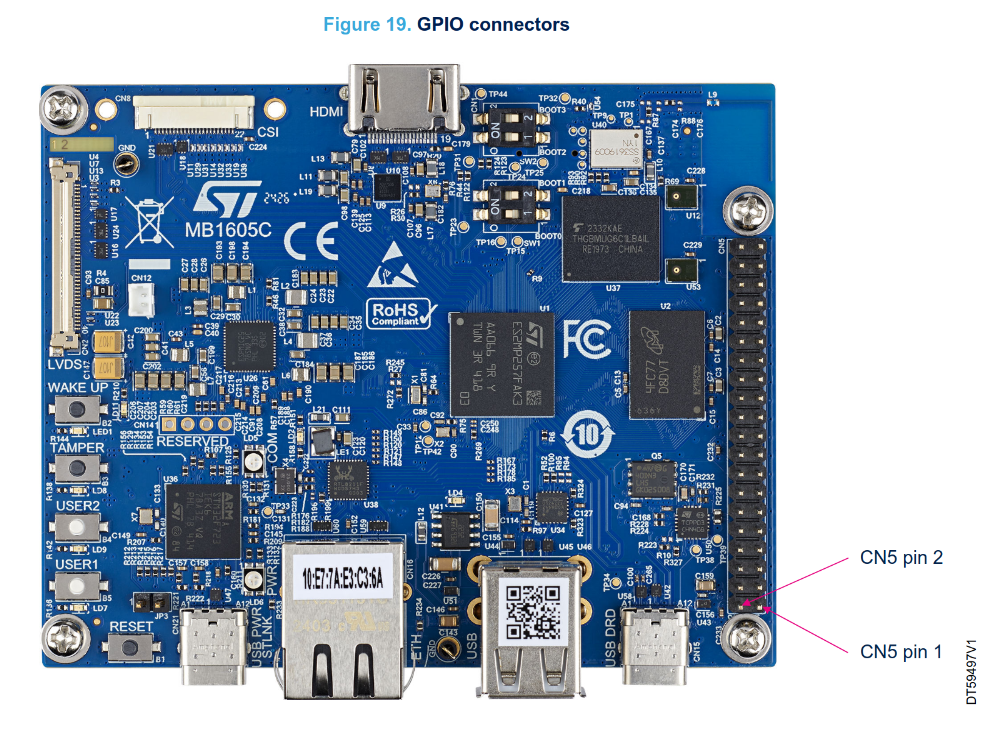
\includegraphics[width=6cm]{labs/sysdev-accessing-hardware-stm32/stm32mp2_pin_map.png}
      \end{center}
      
      \begin{itemize}
      \item Connect one end to pin 7 of connector PF11
      \item Connect the other end to pin 9 (GND) 
      \end{itemize}


      \begin{center}
            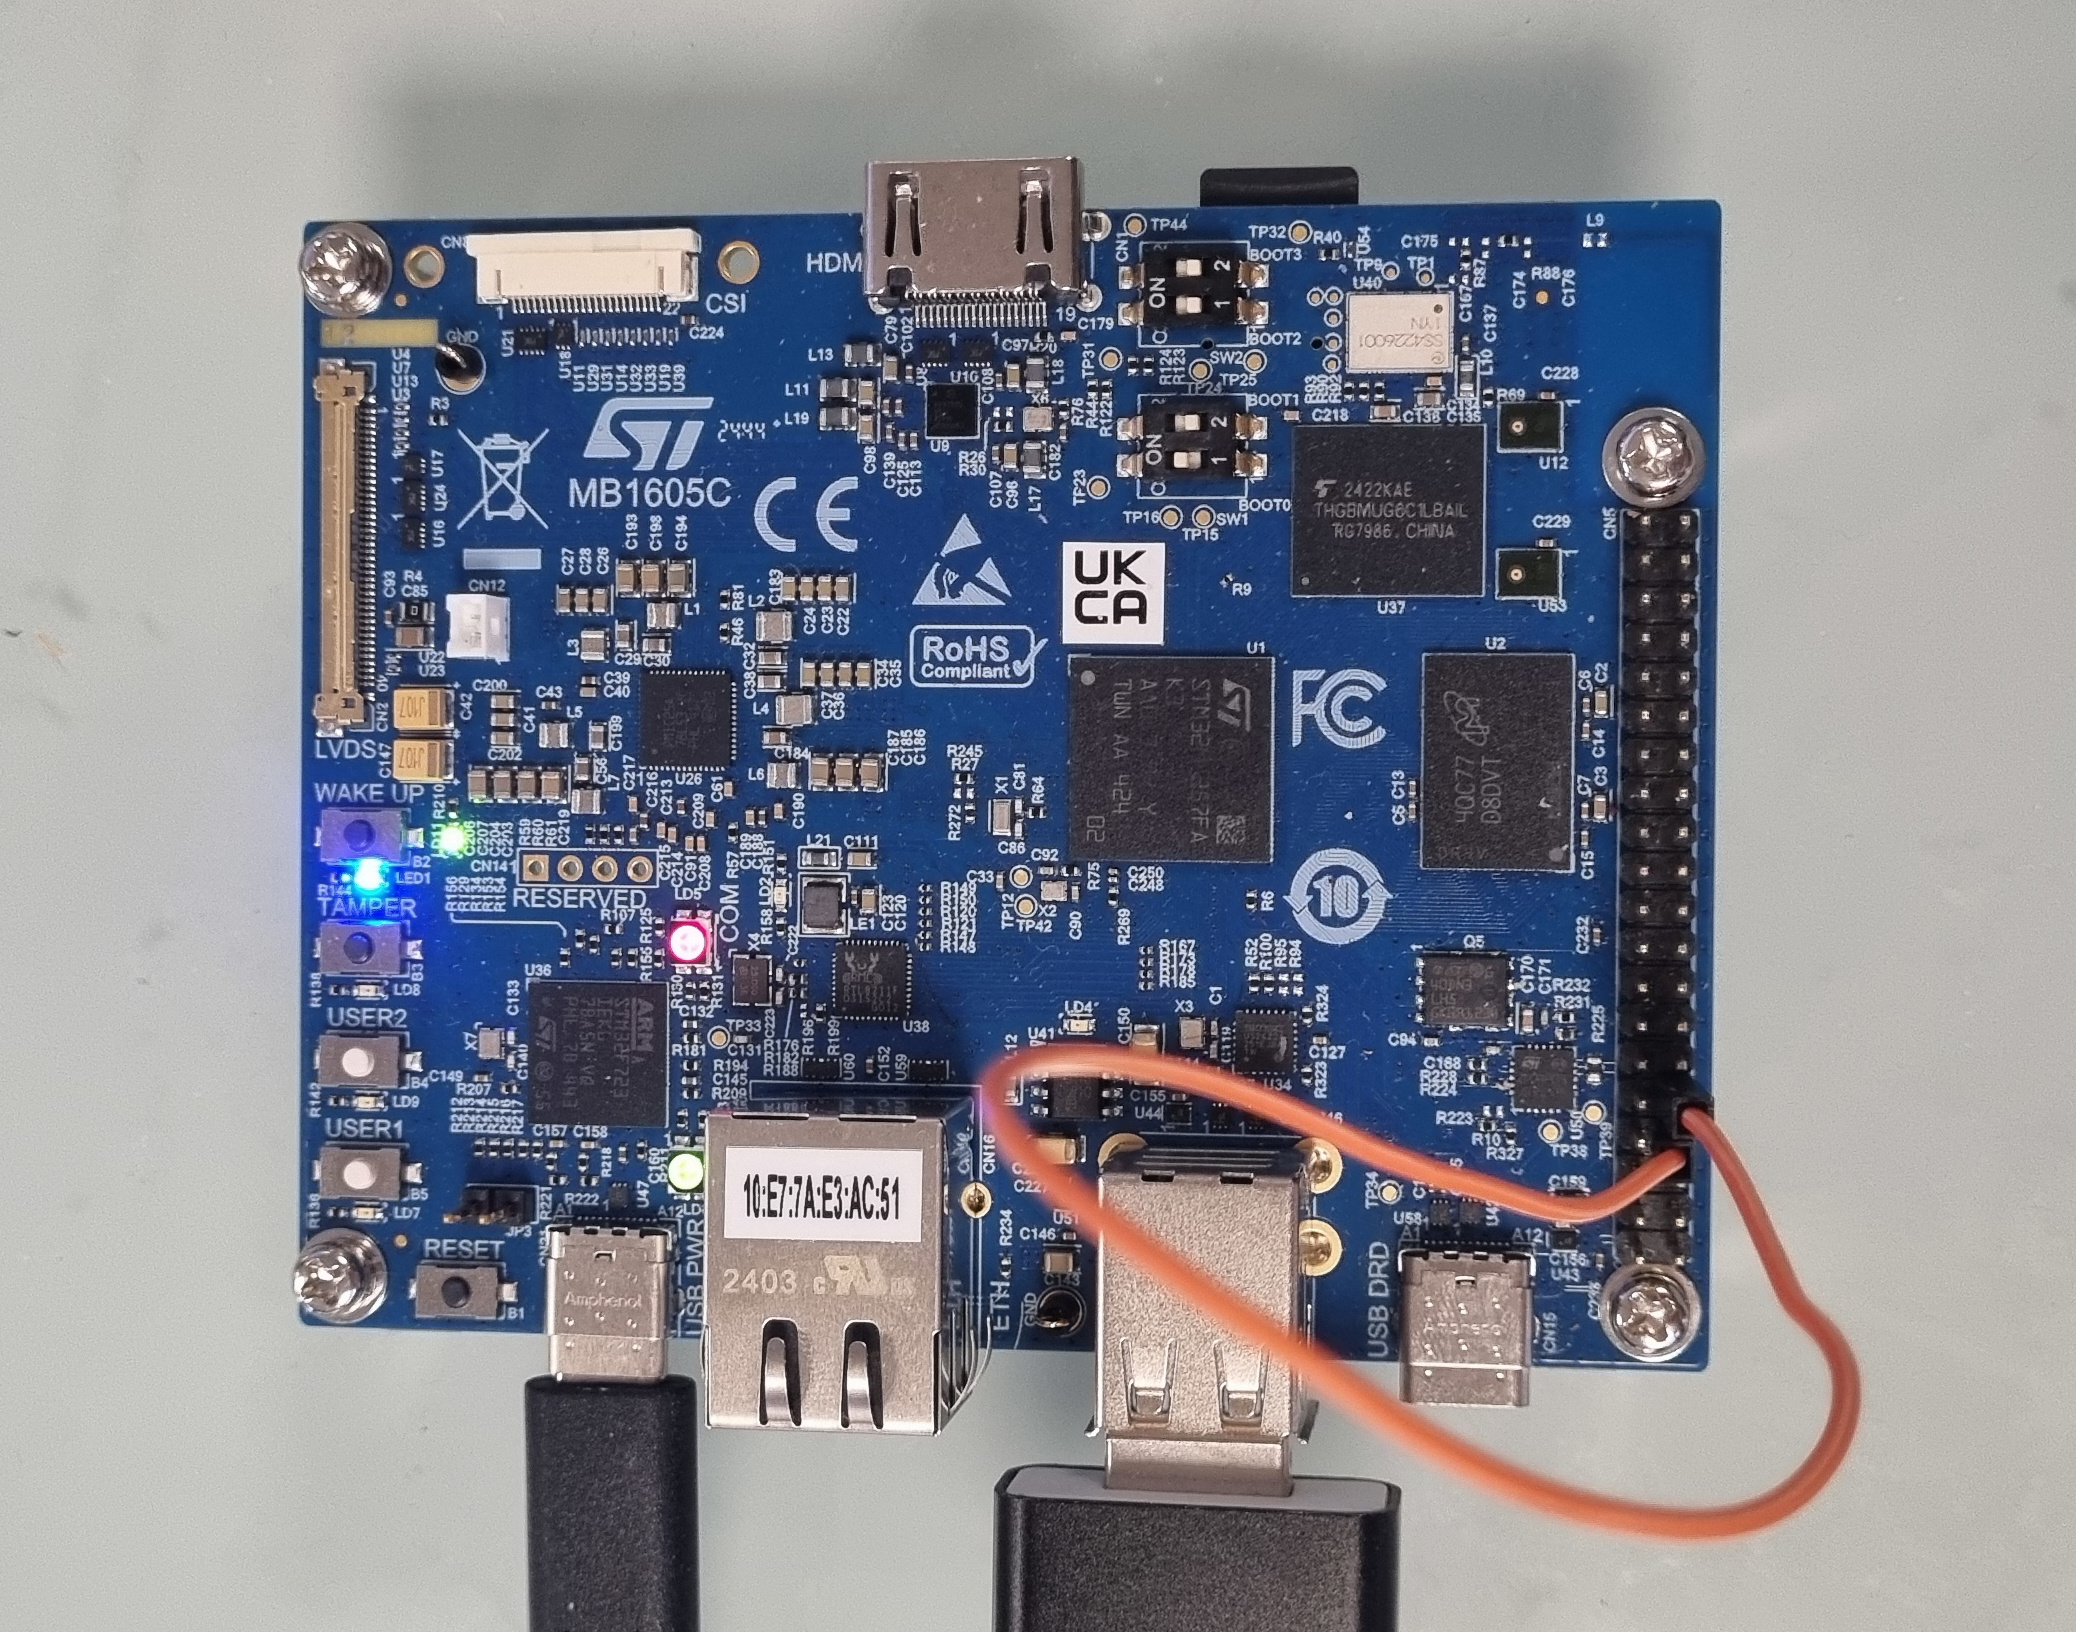
\includegraphics[width=6cm]{labs/sysdev-accessing-hardware-stm32/stm32mp2_gpio_to_gnd.jpg}
      \end{center}
      

      If you check the {\em GPIO expansion connector} table in the board
      documentation
      \footnote{\url{https://www.st.com/en/evaluation-tools/stm32mp257f-dk.html}},
      you will see that the MCO1 pin on the board is connected to the PF11
      STM32 pin. PF11 is actually a GPIO pin on GPIO bank F, and is configured
      as a GPIO by default (no need to change pin muxing to use this pin as
      a GPIO).

      If you get back to the contents of \code{/sys/kernel/debug/gpio}, you'll
      find that GPIO bank F corresponds to \code{gpiochip5} and to GPIO
      numbers 590 to 605. Hence, PF11, the second pin on this bank corresponds to
      GPIO number \gpionum.
\fi

We now have everything we need to drive this GPIO using the legacy
interface. First, let's enable it:

\begin{bashinput}
# cd /sys/class/gpio
# echo %\gpionum% > export
\end{bashinput}

If indeed the pin is still available, this should create a new
\code{\gpioname} file in \code{/sys/class/gpio}.

We can now configure this pin as input:

\begin{bashinput}
# echo in > %\gpioname%/direction
\end{bashinput}

And check its value:

\begin{bashinput}
# cat %\gpioname%/value
0
\end{bashinput}

The value should be \code{0} as the pin is connected to a ground level.
\if\defstring{\labboard}{stm32mp1}
      Now, let's connect our GPIO pin to pin 2 (IOREF 3V3) of connector CN16.
      That's the same connector as before, just the second pin from the top
      (in the board picture above), instead of the seventh one.
\fi
\if\defstring{\labboard}{stm32mp2}
      Now, let's connect our GPIO pin to pin 1 (IOREF 3V3).
\fi
Let's check the value again:

\begin{bashinput}
# cat %\gpioname%/value
1
\end{bashinput}

The value is \code{1} because our pin is connected to a 3.3V level now.

You could use this GPIO to add a button switch to your board, for
example.

Note that you could also configure the pin as output and set its value
through the \code{value} file. This way, you could add an external LED
to your board, for example.

Before moving on to the next section, you can also check
\code{/sys/kernel/debug/gpio} again, and see that {\tt gpio-\gpionum} is now
in use, through the sysfs interface, and is configured as an input pin.

When you're done, you can see your GPIO free:

\begin{bashinput}
# echo %\gpionum% > unexport
\end{bashinput}

\section{Driving LEDs}

First, make sure your kernel is compiled with
\kconfigval{CONFIG_LEDS_CLASS}{y}, \kconfigval{CONFIG_LEDS_GPIO}{y}
,\kconfigval{CONFIG_EXPERT}{y}, \kconfigval{CONFIG_I2C_STM32F7}{y}
and \kconfigval{CONFIG_LEDS_TRIGGER_TIMER}{y}.

Then, go to \code{/sys/class/leds} to see all the LEDs that you are allowed
to control.

Let's control the LED which is called
\code{heartbeat}.

Go into the directory for this LED, and check its trigger (what
routine is used to drive its value):

\begin{bashinput}
# cat trigger
\end{bashinput}

As you can see, there are many triggers to choose from, the current
being \code{heartbeat}, corresponding to the CPU activity.

You can disable all triggers by:

\begin{bashinput}
# echo none > trigger
\end{bashinput}

And then directly control the LED:

\begin{bashinput}
# echo 1 > brightness
# echo 0 > brightness
\end{bashinput}

You could also use the \code{timer} trigger to light the LED
with specified time on and time off:

\begin{bashinput}
# echo timer > trigger
# echo 10 > delay_on
# echo 200 > delay_off
\end{bashinput}
\section{Managing the I2C buses and devices}

\subsection{Enabling an I2C bus}

The next thing we want to do is connect an Nunchuk joystick
to an I2C bus on our board. The I2C bus is very frequently used
to connect all sorts of external devices. That's why we're covering
it here.
\if\defstring{\labboard}{stm32mp1}
      The first task is to find a suitable bus. If you study the
      same document about the board, you will find that only I2C5 is
      conveniently available through the Arduino headers. Let's try
      to use this one!
\fi
\if\defstring{\labboard}{stm32mp2}
      The first task is to find a suitable bus. If you study the
      same document about the board, you will find that only I2C2 and I2C8 are
      conveniently available through the headers pin. Let's try
      to use I2C8!
\fi

First, let's see which I2C buses are already enabled:

\if\defstring{\labboard}{stm32mp1}
      \begin{bashinput}
      # i2cdetect -l
      i2c-1	i2c             STM32F7 I2C(0x5c002000)                 I2C adapter
      i2c-0	i2c             STM32F7 I2C(0x40012000)                 I2C adapter
      \end{bashinput}
\fi
\if\defstring{\labboard}{stm32mp2}
      \begin{bashinput}
      # i2cdetect -l
      i2c-0	i2c       	STM32F7 I2C(0x0000000040130000) 	I2C adapter 
      \end{bashinput}
\fi

\if\defstring{\labboard}{stm32mp1}
      \code{i2c-0} is the I2C controller with registers at
      \code{0x40012000}, which is \code{I2C1} in the STM32MP1
      nomenclature. \code{i2c-1} is the I2C controller with registers at
      \code{0x5c002000}, which is \code{I2C4} in the STM32MP1
      nomenclature. Refer to the STM32MP1 memory map in the datasheet for
      details. Pay attention to the numbering difference: \code{i2c-0},
      \code{i2c-1} is the Linux numbering, based on the registration order
      of enabled I2C busses. Here, because only I2C1 and I2C4 are enabled,
      they are called \code{i2c-0} and \code{i2c-1}.
\fi
\if\defstring{\labboard}{stm32mp2}
      \code{i2c-0} is the I2C controller with registers at
      \code{0x0000000040130000}, which is \code{I2C2} in the STM32MP2
      nomenclature. Refer to the STM32MP25 memory map in the datasheet for
      details.
\fi

\if\defstring{\labboard}{stm32mp1}
      Using the datasheet for the SoC
      \footnote{\url{https://www.st.com/resource/en/reference_manual/dm00327659-stm32mp157-advanced-arm-based-32-bit-mpus-stmicroelectronics.pdf}},
      we can find what is the base address of the registers for the
      \code{I2C5} controller: it is \code{0x40015000}.
\fi
\if\defstring{\labboard}{stm32mp2}
      Using the datasheet for the SoC
      \footnote{\url{https://www.st.com/resource/en/reference_manual/rm0457-stm32mp25xx-advanced-armbased-3264bit-mpus-stmicroelectronics.pdf}},
      we can find what is the base address of the registers for the
      \code{I2C8} controller: it is \code{0x46040000}.
\fi

\subsection{Customizing the Device Tree}

To enable \busname\ on our system, we need to assign set \code{status =
"okay";} in the corresponding Device Tree node.

Fortunately, \busname\ is already defined in the one of the DTS includes
used by the Device Tree for our board. In our case, that's in
\if\defstring{\labboard}{stm32mp1}
      \kfileversion{arch/arm/boot/dts/st/stm32mp151.dtsi}{6.6}. 
\fi
\if\defstring{\labboard}{stm32mp2}
      \kfileversion{arch/arm64/boot/dts/st/stm32mp251.dtsi}{6.6}.
\fi
Look by yourself in this
file, and you will find its definition, but with \code{status =
"disabled";}. This means that this I2C controller is not enabled yet,
and it's up to boards using it to do so.

\if\defstring{\labboard}{stm32mp1}
      We could modify the \kfile{arch/arm/boot/dts/st/stm32mp157a-dk1.dts} file
\fi
\if\defstring{\labboard}{stm32mp2}
      We could modify the \kfile{arch/arm64/boot/dts/st/stm32mp257f-dk.dts} file
\fi
for our board, but that's not a very good idea as this file is
maintained by the kernel developers. The changes that you make could
collide with future changes made by the maintainers for this file.

A more futureproof idea is to create a new Device Tree file which
includes the standard one, and adds custom definitions. So, create a

\if\defstring{\labboard}{stm32mp1}
      new \code{arch/arm/boot/dts/st/stm32mp157a-dk1-custom.dts} file containing:
      \begin{verbatim}
      /dts-v1/;
      #include "stm32mp157a-dk1.dts"
      &i2c5 {
                  status = "okay";
                  /delete-property/ pinctrl-names;
      };
      \end{verbatim}
\fi
\if\defstring{\labboard}{stm32mp2}
      new \code{arch/arm64/boot/dts/st/stm32mp257f-dk-custom.dts} file containing:
      \begin{verbatim}
      /dts-v1/;
      #include "stm32mp257f-dk.dts"
      &i2c8 {
                  status = "okay";
                  /delete-property/ pinctrl-names;
      };
      \end{verbatim}
\fi

As you can see, it's also possible to include \code{dts} files, and not
only \code{dtsi} ones.

Why the \code{/delete-property/} statement? That's because we want
to see what happens when a device doesn't have associated pin
definitions yet.

A device like an I2C controller node is typically declared in the DTSI
files for the SoC, without pin settings as these are board
specific. Pin definitions are then usually defined at board level.

\if\defstring{\labboard}{stm32mp1}
      In our case, we don't see such definitions, but they are actually
      found in the \kfile{arch/arm/boot/dts/st/stm32mp15xx-dkx.dtsi}
      file, shared between multiple stm32mp15 DK boards, which is included
      by the toplevel Device Tree for our board.

      Modify the \kfile{arch/arm/boot/dts/st/Makefile} file to add your custom
\fi
\if\defstring{\labboard}{stm32mp2}
      In our case, we don't see such definitions, but they are actually
      found in the \kfile{arch/arm64/boot/dts/st/stm32mp25xx-dkx.dtsi}
      file, shared between multiple stm32mp25 DK boards, which is included
      by the toplevel Device Tree for our board.

      Modify the \kfile{arch/arm64/boot/dts/st/Makefile} file to add your custom
\fi
Device Tree, and then have it compiled (\code{make dtbs}).

Reboot your board with the update.

\if\defstring{\labboard}{stm32mp1}
      Back to the running system, we can now see that there is one more
      I2C bus. We can also recognize the \busname\ address (\code{0x40015000})
      though it's now associated to the \code{i2c-1} device name, which
      already existed previously, but mapped to a different physical device:

      \begin{bashinput}
      # i2cdetect -l
      i2c-1	i2c             STM32F7 I2C(0x40015000)                 I2C adapter
      i2c-2	i2c             STM32F7 I2C(0x5c002000)                 I2C adapter
      i2c-0	i2c             STM32F7 I2C(0x40012000)                 I2C adapter
      \end{bashinput}
\fi
\if\defstring{\labboard}{stm32mp2}
      Back to the running system, we can now see that there is one more
      I2C bus. We can also recognize the I2C8 address (\code{0x46040000})
      though it's now associated to the \code{i2c-0} device name, which
      already existed previously, but mapped to the I2C2 controller.

      \begin{bashinput}
      # i2cdetect -l 
      i2c-1	i2c       	STM32F7 I2C(0x0000000046040000) 	I2C adapter
      i2c-0	i2c       	STM32F7 I2C(0x0000000040130000) 	I2C adapter
      \end{bashinput}

      Pay attention to the numbering difference: \code{i2c-0},
      \code{i2c-1} is the Linux numbering, based on the registration order
      of enabled I2C busses. Here, because only I2C2 and I2C8 are enabled,
      they are called \code{i2c-0} and \code{i2c-1}.
\fi

\if\defstring{\labboard}{stm32mp1}
      Now, let's use \code{i2cdetect}'s capability to probe a bus for devices.
      Let's start by the bus associated to \code{i2c-2}:

      \begin{verbatim}
      # i2cdetect -r 2
      i2cdetect: WARNING! This program can confuse your I2C bus
      Continue? [y/N] y
      0  1  2  3  4  5  6  7  8  9  a  b  c  d  e  f
      00:          -- -- -- -- -- -- -- -- -- -- -- -- --
      10: -- -- -- -- -- -- -- -- -- -- -- -- -- -- -- --
      20: -- -- -- -- -- -- -- -- 28 -- -- -- -- -- -- --
      30: -- -- -- UU -- -- -- -- -- -- -- -- -- -- -- --
      40: -- -- -- -- -- -- -- -- -- -- -- -- -- -- -- --
      50: -- -- -- -- -- -- -- -- -- -- -- -- -- -- -- --
      60: -- -- -- -- -- -- -- -- -- -- -- -- -- -- -- --
      70: -- -- -- -- -- -- -- --
      \end{verbatim}

      We can see two devices here:
      \begin{itemize}
      \item One at address \code{0x33}, indicated by \code{UU},
            which means that there is a kernel driver actively
            driving this device.
      \item Another one at address \code{0x28}. We just know that
            it's currently not bound to a kernel driver.
      \end{itemize}
\fi
\if\defstring{\labboard}{stm32mp2}
      Now, let's use \code{i2cdetect}'s capability to probe a bus for devices.
      Let's start by the bus associated to \code{i2c-0}:

      \begin{verbatim}
      i2cdetect -r 0
      i2cdetect: WARNING! This program can confuse your I2C bus
      Continue? [y/N] y
      0  1  2  3  4  5  6  7  8  9  a  b  c  d  e  f
      00:          -- -- -- -- -- -- -- -- -- -- -- -- -- 
      10: -- -- -- -- -- -- -- -- -- -- -- -- -- -- -- -- 
      20: -- -- -- -- -- -- -- -- -- -- -- -- -- -- -- -- 
      30: -- -- -- -- -- -- -- -- UU -- -- -- UU UU -- UU 
      40: -- -- -- -- -- -- -- -- -- -- -- -- -- -- -- -- 
      50: -- -- -- -- -- -- -- -- -- -- -- -- -- -- -- -- 
      60: -- -- -- -- -- -- -- -- -- -- -- -- -- -- -- -- 
      70: -- -- -- -- -- -- -- -- 
      \end{verbatim}

      We can see four devices on this internal bus at the addresses \code{0x38}, \code{0x3c}, \code{0x3d}, and \code{0x3f}, indicated by \code{UU},
      which means that a kernel driver is actively managing these devices.
\fi

Now try to probe \busname\ through \code{i2cdetect -r 1}.

You will see that the command will run very slowly because of failing to
connect to the bus. That's because the corresponding signals are
not exposed yet to the outside connectors through pin muxing.

So, get back to your Device Tree and remove the \code{/delete-property/}
line. Recompile your Device Tree and reboot.

You should now be able to probe your bus:

\begin{verbatim}
# i2cdetect -r 1
i2cdetect: WARNING! This program can confuse your I2C bus
Continue? [y/N] y
     0  1  2  3  4  5  6  7  8  9  a  b  c  d  e  f
00:          -- -- -- -- -- -- -- -- -- -- -- -- --
10: -- -- -- -- -- -- -- -- -- -- -- -- -- -- -- --
20: -- -- -- -- -- -- -- -- -- -- -- -- -- -- -- --
30: -- -- -- -- -- -- -- -- -- -- -- -- -- -- -- --
40: -- -- -- -- -- -- -- -- -- -- -- -- -- -- -- --
50: -- -- -- -- -- -- -- -- -- -- -- -- -- -- -- --
60: -- -- -- -- -- -- -- -- -- -- -- -- -- -- -- --
70: -- -- -- -- -- -- -- --
\end{verbatim}

No device is detected yet, because this bus is just
used for external devices. It's time to add one though.

\subsection{Adding and enabling an I2C device}

Let's connect the Nunchuk provided by your instructor
to the \busname\ bus on the board, using breadboard wires:

\begin{center}
\includegraphics[width=4cm]{common/nunchuk-pinout.pdf}
\end{center}

\if\defstring{\labboard}{stm32mp1}
      \includegraphics[width=12cm]{common/dk1-nunchuk-connect.jpg}
      \begin{center}
      \includegraphics[width=6cm]{labs/sysdev-accessing-hardware-stm32/dk1-board-nunchuk-connected.jpg}
      \end{center}

      \begin{itemize}
      \item Connect the Nunchuk PWR pin to pin 4 (3V3) of connector CN16
      \item Connect the Nunchuk GND pin to pin 6 (GND) of connector CN16
      \item Connect the Nunchuk SCL pin to pin 10 (D15 - I2C5\_SCL) of connector CN13
      \item Connect the Nunchuk SDA pin to pin 9 (D14 - I2C5\_SDA) of connector CN13
      \end{itemize}
\fi
\if\defstring{\labboard}{stm32mp2}
      \begin{center}
      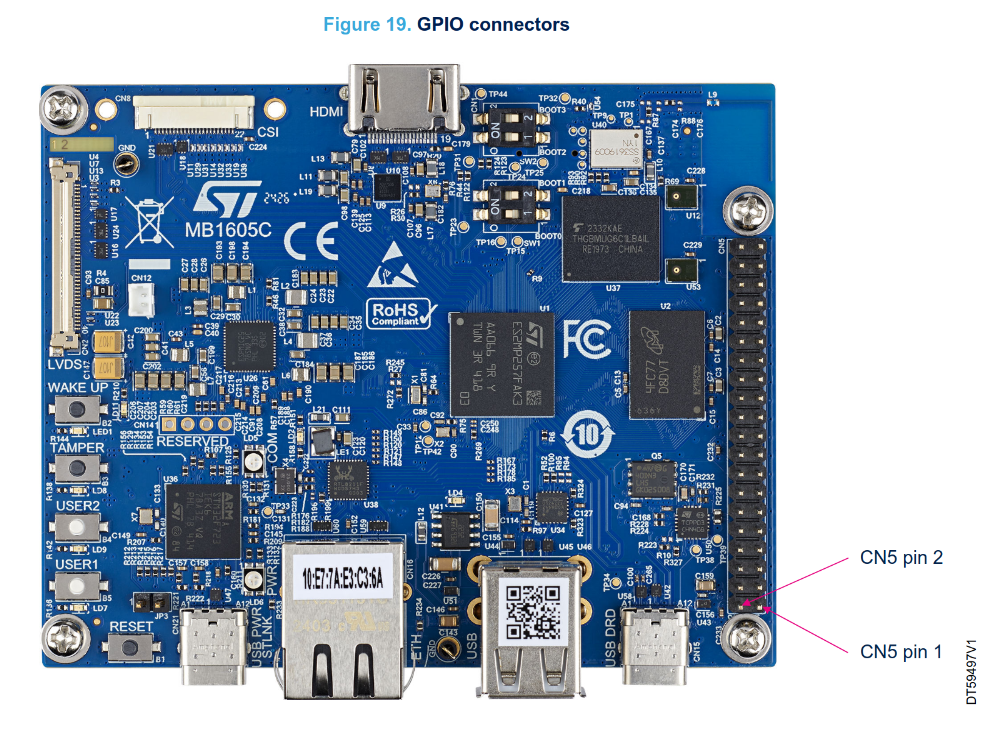
\includegraphics[width=10cm]{labs/sysdev-accessing-hardware-stm32/stm32mp2_pin_map.png}
      
      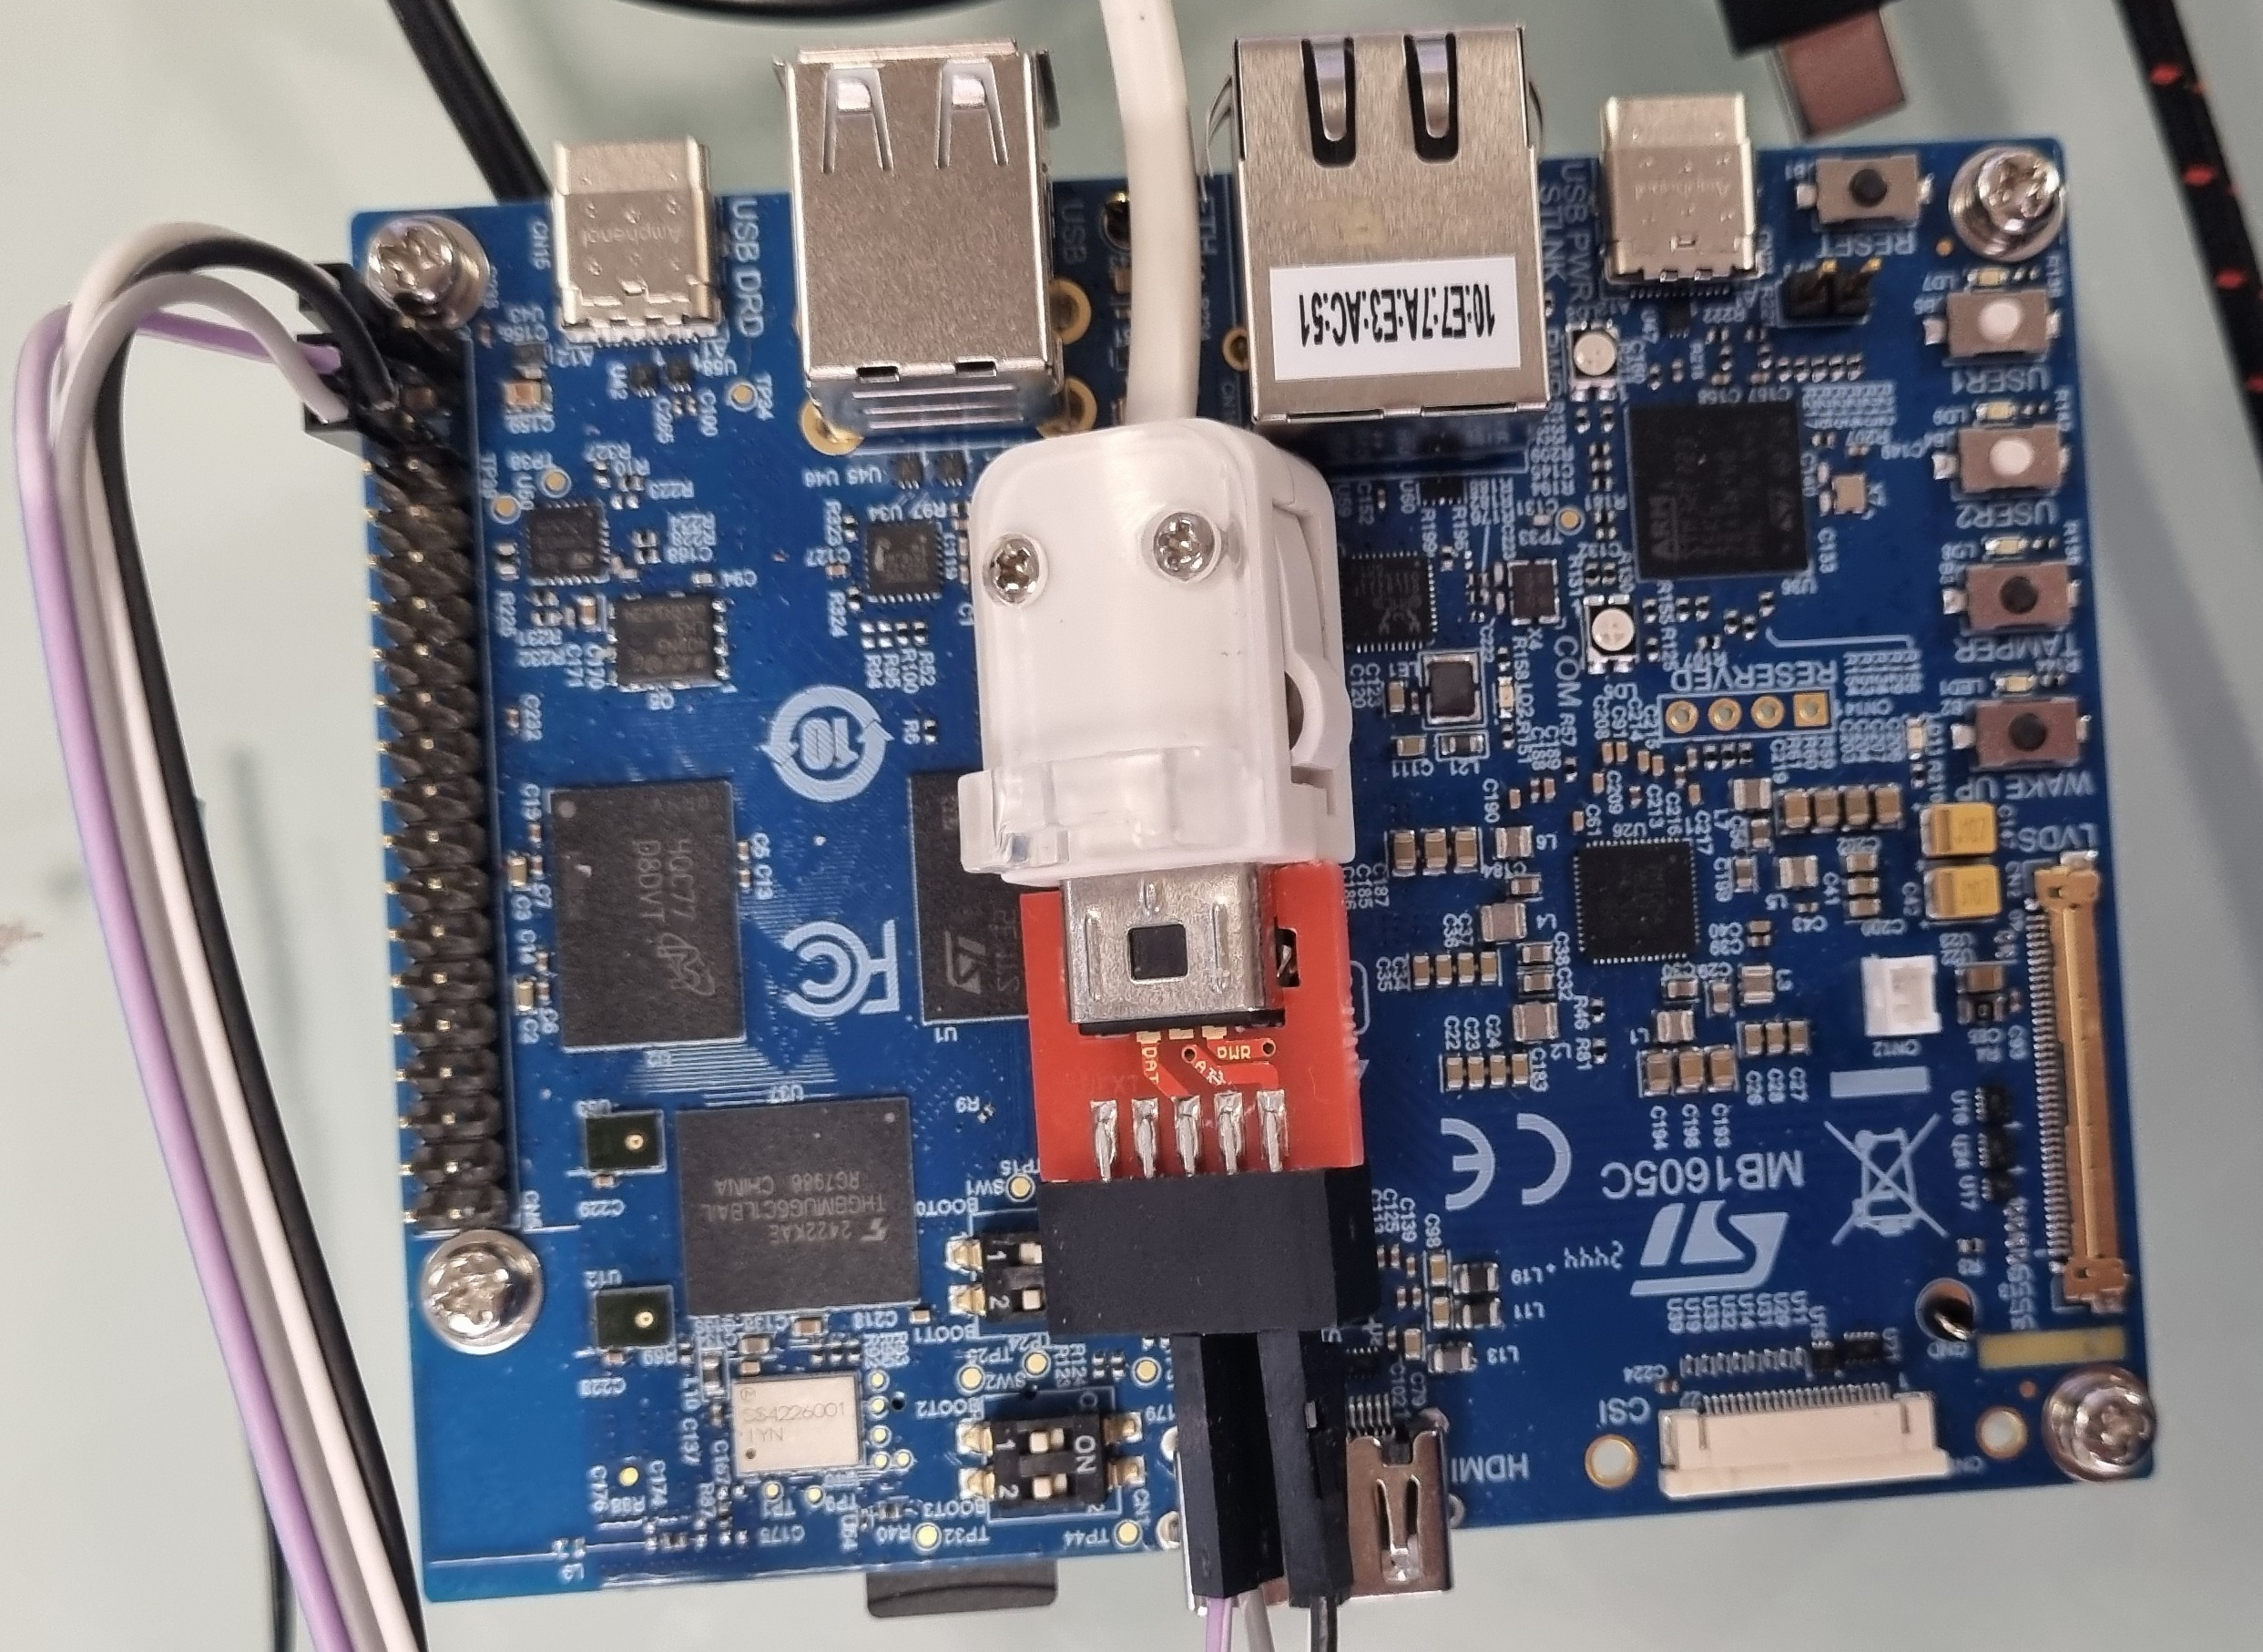
\includegraphics[width=6cm]{labs/sysdev-accessing-hardware-stm32/stm32mp2_nunchuk.jpg}
      \end{center}

      \begin{itemize}
      \item Connect the Nunchuk PWR pin to pin 1 (3V3).
      \item Connect the Nunchuk GND pin to pin 6 (GND).
      \item Connect the Nunchuk SCL pin to pin 5 (PZ4 - I2C8\_SCL).
      \item Connect the Nunchuk SDA pin to pin 3 (PZ3 - I2C8\_SDA).
      \end{itemize}
\fi

If you didn't do any mistake, your new device should be detected at
address \code{0x52}:

\begin{verbatim}
# i2cdetect -r 1
i2cdetect: WARNING! This program can confuse your I2C bus
Continue? [y/N] y
     0  1  2  3  4  5  6  7  8  9  a  b  c  d  e  f
00:          -- -- -- -- -- -- -- -- -- -- -- -- --
10: -- -- -- -- -- -- -- -- -- -- -- -- -- -- -- --
20: -- -- -- -- -- -- -- -- -- -- -- -- -- -- -- --
30: -- -- -- -- -- -- -- -- -- -- -- -- -- -- -- --
40: -- -- -- -- -- -- -- -- -- -- -- -- -- -- -- --
50: -- -- 52 -- -- -- -- -- -- -- -- -- -- -- -- --
60: -- -- -- -- -- -- -- -- -- -- -- -- -- -- -- --
70: -- -- -- -- -- -- -- --
\end{verbatim}

We will later compile an out-of-tree kernel module to support this device.

\section{Plugging a USB audio headset}

In the next labs, we are going to play audio using a USB audio headset.
Let's see whether our kernel supports such hardware by plugging the
headset provided by your instructor.

Before plugging the device, look at the output of \code{lsusb}:

\if\defstring{\labboard}{stm32mp1}
      \begin{bashinput}
      # lsusb
      Bus 002 Device 002: ID 0424:2514
      Bus 001 Device 001: ID 1d6b:0002
      Bus 002 Device 001: ID 1d6b:0002
      \end{bashinput}
\fi
\if\defstring{\labboard}{stm32mp2}
      \begin{bashinput}
      # lsusb 
      Bus 001 Device 001: ID 1d6b:0002 Linux 6.6.48-g3682d604ecbd ehci_hcd EHCI Host Controller
      Bus 001 Device 002: ID 0424:2422 
      \end{bashinput}
\fi
Now, when you plug the USB headset, a number of messages should appear
on the console, and running \code{lsusb} again should show an
additional device:

\if\defstring{\labboard}{stm32mp1}
      \begin{bashinput}
      # lsusb
      Bus 002 Device 004: ID 0d8c:0014
      Bus 002 Device 002: ID 0424:2514
      Bus 001 Device 001: ID 1d6b:0002
      Bus 002 Device 001: ID 1d6b:0002
      \end{bashinput}
\fi
\if\defstring{\labboard}{stm32mp2}
      \begin{bashinput}
      # lsusb 
      Bus 001 Device 001: ID 1d6b:0002 Linux 6.6.48-g3682d604ecbd ehci_hcd EHCI Host Controller
      Bus 001 Device 003: ID 1b3f:2008 GeneralPlus USB Audio Device
      Bus 001 Device 002: ID 0424:2422 
      \end{bashinput}
\fi

You can see the vendor and product ID in the form \code{1a2b:1234}.
Of course, this depends on the actual USB audio device
that you used.

The device also appears in \code{/sys/bus/usb/devices/}, in a
directory whose name depends on the topology of the USB bus. When the
device is plugged in the kernel messages show:

\begin{bashinput}
usb 1-1.X: new full-speed USB device number X using ehci-platform
\end{bashinput}

So if we go in \code{/sys/bus/usb/devices/1-1.X}, we get the {\em
sysfs} representation of this USB device:

\begin{bashinput}
# cd /sys/bus/usb/devices/1-1.X
# cat idVendor
1a2b
# cat idProduct
1234
# cat manufacturer
C-Media Electronics Inc.
# cat product
USB Audio Device
\end{bashinput}

However, while the USB device is detected, we currently do not have
any driver for this device, so no actual sound card is detected.

\section{Enabling, installing and using in-tree kernel modules}

Go back to the kernel source directory.

The Linux kernel has a generic driver supporting all USB audio devices
supporting the standard USB audio class. This driver can be enabled
using the \kconfig{CONFIG_SND_USB_AUDIO} configuration option. Look
for this parameter in the kernel configuration, and you should find
that it is already enabled as a module.

So, instead of compiling the corresponding driver as a built-in, that's
a good opportunity to practice with kernel modules.

So, compile your modules:
\begin{bashinput}
make modules
\end{bashinput}

Then, following details given in the lectures, install the modules in our NFS
root filesystem (\code{$HOME/__SESSION_NAME__-labs/tinysystem/nfsroot}).

Also make sure to update the kernel image (\code{make zImage}), and reboot the
board.  Indeed, due to the changes we have made to the kernel source code,
the kernel version is now {\tt \workingkernel.<x>-dirty}, the {\em dirty}
keyword indicating that the Git working tree has uncommitted changes.
The modules are therefore installed in {\tt /lib/modules/\workingkernel.<x>-dirty/},
and the version of the running Linux kernel must match this.

After rebooting, try to load the module that we need:

\begin{bashinput}
modprobe snd-usb-audio
\end{bashinput}

By running \code{lsmod}, see all the module dependencies that
were loaded too.

You can also see that a new USB device driver in
\code{/sys/bus/usb/drivers/snd-usb-audio}. This directory shows which
USB devices are bound to this driver.

You can check that \code{/proc/asound} now exists (thanks to loading
modules for ALSA, the Linux sound subsystem), and that one sound
card is available:

\begin{bashinput}
# cat /proc/asound/cards
 0 [Device         ]: USB-Audio - USB Audio Device
                      C-Media Electronics Inc. USB Audio Device at usb-5800d000.usb-1.1, full speed
\end{bashinput}

Check also the \code{/dev/snd} directory, which should now contain
some character device files. These will be used by the user-space
libraries and applications to access the audio devices.

Modify your startup scripts so that the \code{snd-usb-audio} module
is always loaded at startup.

We cannot test the sound card yet, as we will need to build some
software first. Be patient, this is coming soon.

\section{Compiling and installing an out-of-tree kernel module}

The next device we want to support is the I2C Nunchuk. There is a driver
in the kernel to support it when connected to a Wiimote controller, but
there is no such driver to support it as an I2C device.

Fortunately, one is provided in
\code{$HOME/__SESSION_NAME__-labs/hardware/data/nunchuk/nunchuk.c}. You can check
\href{https://bootlin.com/training/kernel/}{Bootlin's Linux kernel and
driver development course} to learn how to implement all sorts of device
drivers for Linux.

Go to this directory, and compile the out-of-tree module as follows:

\begin{bashinput}
make -C $HOME/__SESSION_NAME__-labs/kernel/linux M=$PWD
\end{bashinput}

Here are a few explanations:
\begin{itemize}
\item The \code{-C} option lets \code{make} know which Makefile to
      use, here the toplevel Makefile in the kernel sources.
\item \code{M=$PWD} tells the kernel Makefile to build external
      module(s) from the file(s) in the current directory.
\end{itemize}

Now, you can install the compiled module in the NFS root filesystem
by passing the \code{modules_install} target and specifying the
target directory through the \code{INSTALL_MOD_PATH} variable:

\begin{bashinput}
make -C $HOME/__SESSION_NAME__-labs/kernel/linux \
     M=$PWD \
     INSTALL_MOD_PATH=$HOME/__SESSION_NAME__-labs/tinysystem/nfsroot \
     modules_install
\end{bashinput}

You can see that this installs out-of-tree kernel modules under
\code{lib/modules/<version>/updates/}.

Back on the target, you can now check that your custom module can
be loaded:

\begin{bashinput}
# modprobe nunchuk
[ 4317.737978] nunchuk: loading out-of-tree module taints kernel.
\end{bashinput}

See \kdochtml{kbuild/modules} in kernel documentation
for details about building out-of-tree kernel modules.

However, run \code{i2cdetect -r 1} again. You will see that the
Nunchuk is still detected, but still not driven by the kernel.
Otherwise, it would be signaled by the \code{UU} character. You
may also look at the \code{nunchuk.c} file and notice a
\code{Nunchuk device probed successfully} message that you didn't
see when loading the module.

That's because the Linux kernel doesn't know about the Nunchuk
device yet, even though the driver for this kind of devices is
already loaded. Our device also has to be described in the Device Tree.

You can confirm this by having a look at the contents of the
\code{/sys/bus/i2c} directory.  It contains two subdirectories:
\code{devices} and \code{drivers}.

In \code{drivers}, there should be a \code{nunchuk} subdirectory,
but no symbolic link to a device yet. In \code{devices} you should
see some devices, but not the Nunchuk one yet.

\section{Declaring an I2C device}

To allow the kernel to manage our Nunchuk device, let's declare the
device in the custom Device Tree for our board. The declaration of the \busname\ 
bus will then look as follows:

\if\defstring{\labboard}{stm32mp1}
      \begin{verbatim}
      &i2c5 {
            status = "okay";
            clock-frequency = <100000>;

            nunchuk: joystick@52 {
                  compatible = "nintendo,nunchuk";
                  reg = <0x52>;
            };
      };
      \end{verbatim}
\fi
\if\defstring{\labboard}{stm32mp2}
      \begin{verbatim}
      &i2c2 {
              status = "okay";
              clock-frequency = <100000>;
      
              nunchuk: joystick@52 {
                      compatible = "nintendo,nunchuk";
                      reg = <0x52>;
              };
      };
      \end{verbatim}
\fi

Here are a few notes:
\begin{itemize}
\item The \code{clock-frequency} property is used to configure the bus
      to operate at 100 KHz. This is supposed to be required for the
      Nunchuk.
\item The Nunchuk device is added through a child node in the I2C
      controller node.
\item For the kernel to {\em probe} and drive our device, it's required
      that the \code{compatible} string matches one of the
      \code{compatible} strings supported by the driver.
\item The \code{reg} property is the address of the device on the
      I2C bus. If it doesn't match, the driver will probe the device
      but won't be able to communicate with it.
\end{itemize}

Recompile your Device Tree and reboot your kernel with the new binary.

You can now load your module again, and this time, you should see that
the Nunchuk driver probed the Nunchuk device:

\begin{bashinput}
# modprobe nunchuk
[   66.680455] nunchuk: loading out-of-tree module taints kernel.
[   66.687645] input: Wii Nunchuk as /devices/platform/soc/40015000.i2c/i2c-1/1-0052/input/input3
[   66.695421] Nunchuk device probed successfully
\end{bashinput}

List the contents of \code{/sys/bus/i2c/drivers/nunchuk} once again. You
should now see a symbolic link corresponding to our new device.

Also list \code{/sys/bus/i2c/devices/} again. You should now see the
Nunchuk device, which can be recognized through its \code{0052} address.
Follow the link and you should see a symbolic link back to the Nunchuk
driver!

We are not ready to use this input device yet, but at least we can test
that we get bytes when buttons or the joypad are used. In the below
command, use the same number as in the message you got in the console
(\code{event3} for \code{input3} for example):

\begin{bashinput}
# cat /dev/input/event3 | od -x
\end{bashinput}

{\bf Caution}: using \code{od} directly on input event files should
work but is currently broken with the Musl library. We are investigating
this issue.

We will use the Nunchuk to control audio playback in an upcoming lab.

\section{Setting the board's model name}

Modify the custom Device Tree file one last time to override the model
name for your system. Set the \code{model} property to
\labboard\ media player. Don't hesitate to ask your
instructor if you're not sure how.

Recompile the device tree, and reboot the board with it. You should see
the new model name in two different places:

\begin{itemize}
\item In the first kernel messages on the serial console.
\item In \code{/sys/firmware/devicetree/base/model}. This can be
      handy for a distribution to identify the device it's running on.
      By the way, you can explore \code{/sys/firmware/devicetree} and
      find that every subdirectory corresponds to a DT node, and every
      file corresponds to a DT property.
\end{itemize}

\section{Committing kernel tree changes}

Now that our changes to the kernel sources are over,
create a branch for your changes and create a patch for them.
{\bf Please don't skip this step} as we need it for the next labs.

First, if not done yet, you should set your identity
and e-mail address in git:

\begin{bashinput}
git config --global user.email "linus@bootlin.com"
git config --global user.name "Linus Torvalds"
\end{bashinput}

This is necessary to create a commit with the \code{git commit -s}
command, as required by the Linux kernel contribution guidelines.

Let's create the branch and the patch now:

\if\defstring{\labboard}{stm32mp1}
      \begin{bashinput}
      git checkout -b bootlin-labs
      git add arch/arm/boot/dts/st/stm32mp157a-dk1-custom.dts arch/arm/boot/dts/st/Makefile
      git commit -as -m "Custom DTS for Bootlin lab"
      \end{bashinput}

      We can now create the patch:\\
      \texttt{git format-patch stable/linux-\workingkernel.y}
\fi
\if\defstring{\labboard}{stm32mp2}
      \begin{bashinput}
      git checkout -b bootlin-labs
      git add arch/arm64/boot/dts/st/stm32mp257f-dk-custom.dts arch/arm64/boot/dts/st/Makefile
      git commit -as -m "Custom DTS for Bootlin lab"
      \end{bashinput}
      
      We can now create the patch:\\
      \texttt{git format-patch v6.6-stm32mp-r1}
\fi

This should generate a \code{0001-Custom-DTS-for-Bootlin-lab.patch}
file.

Creating the branch will impact the versions of the kernel and the modules.
Compile your kernel and install your modules again (not necessary for the
Nunchuk one for the moment) and see the version changes through the
new base directory for modules.

To save space for the next lab, remove the old directory under
\code{lib/modules} containing the "dirty" modules.

Don't forget to update the kernel your board boots.

That's all for now!
